\section{Komplette grafer}
En komplet graf er en graf hvor et hvert unikt par af knuder i grafen er forbundet.
En komplet graf navngives $K_n$ hvor $n$ er antallet af knuderf i grafen.
I figur \ref{fig:komplette_grafer} ses de første 5 komplette grafer.
En graf hvor mindst ét par af knuder ikke er forbundet, kaldes en ikke-komplet graf.

\begin{figure}[h]
	\centering
	% Radius of regular polygons
\newdimen\R
\R=1cm

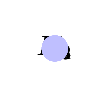
\begin{tikzpicture}[thick]
  \foreach \x in {1,2,3,4,5}{
    \node[yshift=-1.5\R, xshift=\x*2.5\R-2.5\R] {$K_\x $} {};
  }
  \begin{scope}[every node/.style={circle,fill=blue!25}]
    \node (0:0) {};

    \foreach \x in {1,2}{
      \node[xshift=2.5\R] (\x) at (\x*180-180:\R) {};
    }
    \path (1) edge (2);

    \foreach \x in {1,2,3}{
      \node[xshift=5\R] (\x) at (\x*120-120:\R) {};
    }
    \path (1) edge (2);
    \path (2) edge (3);
    \path (3) edge (1);
  
    \foreach \x in {1,2,3,4}{
      \node[xshift=7.5\R] (\x) at (\x*90-90:\R) {};
    }
    \foreach \x in {1,2,3}{
      \path (4) edge (\x);
    }
    \foreach \x in {1,2}{
      \path (3) edge (\x);
    }
    \path (1) edge (2);
  
    \foreach \x in {1,2,3,4,5}{
      \node[xshift=10\R] (\x) at (\x*72-72:\R) {};
    }
    \foreach \x in {1,2,3,4}{
      \path (5) edge (\x);
    }
    \foreach \x in {1,2,3}{
      \path (4) edge (\x);
    }
    \foreach \x in {1,2}{
      \path (3) edge (\x);
    }
    \path (1) edge (2);
  \end{scope}
\end{tikzpicture}

	\caption{De første $5$ komplette grafer} \label{fig:komplette_grafer}
\end{figure}

Antallet af kanter i en komplet graf $K_n$ afhænger kun af $n$.

\begin{thm}
	For en komplet graf $K_n = (V_n, E_n)$ med $n$ knuder er $|E_n|$ antallet af kanter. Da er
	\begin{align*}
		|E_n| = \frac{n (n - 1)}{2}
	\end{align*}
\end{thm}
\begin{proof}
	For at gennemføre et induktionsbevis skal basisskridtet og induktionsskridtet gennemføres.
	Lad propositionen $P(n)$ være at $|E_n|= \frac{n (n - 1)}{2}$, hvor $n$ er antal knuder i en komplet graf $K_n$ og $m$ være antal kanter.

	\textit{Basisskridt:} $K_1$ består af en enkelt knude, og da der ikke er et par af knuder i grafen, må der da ikke eksistere nogen kanter.
	$\frac{ 1 \cdot 0}{2} = 0$, hvilket betyder at $P(1)$ er sand. Da er basisskidtet gennemført.

	\textit{Induktionsskridt:} Det skal nu vises at der for et vilkårligt $k$ gælder at $P(k) \to P(k + 1)$, altså at $|E_k| = \frac{k (k - 1)}{2}$ medfører at $|E_{k+1}| = \frac{k (k + 1)}{2}$.

	Antag at $|E_k| = \frac{k (k - 1)}{2}$ for $K_k$.
	Den næste komplette graf $K_{k+1}$ må være den graf hvor der er én til knude. Denne nye knude $v$ skal være forbundet til alle knuder i $K_k$ for at være en komplet graf. $\deg (v)$ må da være lig $k$. Da må
	\begin{align*}
		|E_{k+1}| 
		&= |E_k| + k \\
		&= \frac{k (k - 1)}{2} + k \\
		&= \frac{k^2 - k}{2} + \frac{2k}{2} \\
		&= \frac{k^2 + k}{2} \\
		&= \frac{k (k + 1)}{2}
	\end{align*}
	Dette er netop $P(k + 1)$, hvilket betyder at induktionsskridtet er gennemført.
\end{proof}
